\documentclass[twocolumn]{article}

\usepackage{tikz}
\usepackage{amsmath}
\usepackage{biblatex}
\usepackage{neuralnetwork}
\usepackage[plain]{fancyref}

\usetikzlibrary{shapes}
\usetikzlibrary{arrows}
\usetikzlibrary{positioning}
\usetikzlibrary{calc}

\addbibresource{speakerRecognition.bib}

\title{Speaker Recognition Using Artificial Neural Networks}

\author{
  Omar Emara (20180364), Mohamed Alkhateb (20180470), Karim Ashraf (20180424) \\
  Mohamed Samir (20180503), Ahmed Mohamed (20170772) \\
}

\begin{document}

\maketitle

\begin{abstract}

  Humans are rather good at identifying a person by their voice. This ability
  is attributed to the large variation in the physiology of the human vocal
  systems and the development of special regions in the human brain that learns
  to distinguish between voices. While the ability to recognize voices comes
  natural to humans, the same couldn't be said about machines. Thus scientist
  in the field of artificial intelligence have long yearned to develop methods
  of \emph{Speaker Recognition}. The advance of neural networks in the field of
  artificial intelligence has certainly helped tremendously to achieved this
  goal. In \Fref{sec:Introduction}, we will introduce the concept of speaker
  recognition systems, classify speaker recognition systems, and describe the
  physiology of sound production in humans. In \Fref{sec:RecognitionSystems},
  we will describe the components that make a speaker recognition system,
  introduce some of the methods used to to implement those components, and
  review the literature on the topic. In \Fref{sec:Implementation}, we will
  introduce our implementation of the system and compare it to the available
  systems. Finally, the article is concluded in \Fref{sec:Conclusion}.

\end{abstract}

\section{Introduction}
\label{sec:Introduction}

\subsection{Definition}

There are many definitions for speaker recognition due to the multitude of
applications where it is employed. However, generally, a speaker recognition
system is a system that can distinguish between human voices and make decisions
based on that distinction like classification, verification, or other
decisions. Speaker recognition systems can be classified to three classes as
demonstrated in the following sections.

\subsubsection{Speaker Verification}

\emph{Speaker Verification} systems are systems that can verify a certain
identity claim. Those systems are sometimes called one to one speaker
recognition. In those systems, one makes a claim that one is a certain person
providing a voice sample as a proof of the claim. The system then compares this
voice sample with a stored \emph{model} or \emph{template} that the system
previously generated. Finally, the system either accepts or rejects the claim.
The main application for this system is access control systems, where the
verification is used to grant access to a certain resource.

\subsubsection{Speaker Identification}

\emph{Speaker identification} systems try to identify a person whose voice
sample is provided from a set of known set of persons that are stored as
\emph{models} or \emph{templates}.  Such systems are sometimes called one to
many speaker recognition. The set of persons can be classified as \emph{Open
Set} or \emph{Closed Set}. A closed set is a set where the voice sample is
guaranteed to match one model from the set. On the other hand, an open set is a
set where no such guarantee exist. One application for this system is labeling
multi-speaker data as explained in the following section.

\subsubsection{Speaker Detection}

\emph{Speaker Detection} was introduced by the National Institute of Standards
and Technology (\emph{NIST}) in \autocite{Przybocki1999}. Such systems are
concerned with open set speaker identification for conversational data such as
telephone conversations. This conversational data is typically multi-speaker,
so it is essential that the system be able to perform speaker tracking and
labeling. That is, the system should be able to segment the conversation into
segments that are produced by each person in the conversation and label those
segments using a speaker identification system as explain before. Many such
systems were constructed, namely \autocite{Wilcox1994} and
\autocite{Delacourt2000}.

\subsubsection{Text Dependence}

Aside from the aforementioned classification. It is possible to classify a
speaker recognition system as either \emph{Text Depended} or \emph{Text
Independent}. A text dependent system assumes the voice samples spell a certain
text while a text independent system make no assumptions about the spelled
text. A text dependent system is typically more accurate, but in reality, such
systems are not popular because in most applications the text is not known.
Authentication systems, however, can make this assumption because the user
records and inputs the voice sample real-time and voluntarily.

\subsection{Physiology}

Before going into the details of the speaker recognition system, it is
important to recognize the physiology of the voice production system in humans.
Human voice production systems are characterized by their large variation
across speakers, be it physiological or behavioral. For instance, the size of
the \emph{Glottis} and \emph{Vocal Tract} determine the \emph{Fundamental
Frequency} of the produced voice. The mean fundamental frequency for males is
approximately 100 Hz, for females 200 Hz, and for children 300 Hz. Thus, it is
possible to classify the speaker by sex and age by measuring the fundamental
frequency of their voice sample. Moreover, the fundamental frequency also
varies across speakers of the same sex and age, albeit a small variation, so
more information is needed to make a better prediction.

The human voice production system is called the \emph{Speech Apparatus}. It is
composed of many organs including the lungs, larynx, lower jaw, tongue, lips,
and the velum. The process of producing voice is rather complicated and a high
level modeling of the apparatus is usually employed to simplify the
conceptualization process. Two such models are usually suggested. An
\emph{Acoustic Model} as that described by \autocite{Maeda1982} which describe
the apparatus using a group of differential equation and can be reversed using
numerical integration. However, the model we will be using in this article is a
\emph{Source-Filter} model. In this model, the organs are classified into two
groups, \emph{Phonatory Organs} and \emph{Articulatory Organs}. Phonatory
organs include the lungs and larynx and they are viewed as the source of voice
production. Articulatory organs include the lower jaw, tongue, lips, and the
velum and they are viewed as organs of modulation or as a filter of the voice
produced at the phonatory organs. A detailed description and analysis of this
model is introduced in \autocite{Degottex2010}. The importance of this model
will become apparent in \Fref{sec:FeatureExtraction}.

\section{Recognition Systems}
\label{sec:RecognitionSystems}

\subsection{System Architecture}

The architecture of a traditional speaker recognition system is illustrated in
\Fref{fig:SystemArchitecture}. Essentially, a voice sample is input into the
system. Then the system tries to extract useful \emph{features} from the input.
Next, the system tries to match the extracted features with the models it
already has stored. Finally, the system makes a decision in the form of a claim
verification or an identification. Each of those steps are described in one of
the following sections.

\begin{figure}
\begin{center}
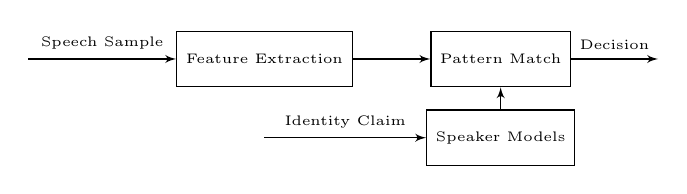
\begin{tikzpicture}[auto, node distance = 3cm, > = latex', font = \tiny]
\tikzset{
  block/.style = {draw, fill = white, rectangle, minimum height = 2em},
  input/.style = {coordinate},
  output/.style = {coordinate},
}
\node [input] (speechSample) {};
\node [block, right of = speechSample] (featureExtraction) {Feature Extraction};
\node [block, right of = featureExtraction] (patternMatch) {Pattern Match};
\node [block, below of = patternMatch, node distance = 1cm] (speakerModels) {Speaker Models};
\node [input, left of = speakerModels] (identityClaim) {};
\node [output, right of = patternMatch, node distance = 2cm] (decision) {};
\draw [->] (speechSample) -- node{Speech Sample} (featureExtraction);
\draw [->] (featureExtraction) -- (patternMatch);
\draw [->] (speakerModels) -- (patternMatch);
\draw [->] (identityClaim) -- node{Identity Claim} (speakerModels);
\draw [->] (patternMatch) -- node{Decision} (decision);
\end{tikzpicture}
\end{center}
\caption{The architecture of a general speaker recognition system.}
\label{fig:SystemArchitecture}
\end{figure}

\subsection{Feature Extraction}
\label{sec:FeatureExtraction}

The system receives a digital sound signal, which is nothing more than a number
of samples sampled at different times at a certain rate called the
\emph{Sampling Rate}. It is very difficult to use this raw signal in pattern
matching, so a different representation of the signal is needed. The process of
finding this representation is called \emph{Feature Extraction}. We can broadly
classify the features we can extract into \emph{High-Level Features} and
\emph{Low-Level Features}.

\subsubsection{High-Level Features}

High-level features in the context of speech processing usually means
linguistic features. Such as the words used in the speech, the frequency of the
used words, the pauses that the speaker makes, and so on. Those features are
not very useful in most applications because they require long speeches to
extract meaningful information. Moreover, they are subject to voluntary
variations in speech. For instance, one can change the way one speaks to get
around speaker identification systems that matches high-level features.

\subsubsection{Low-Level Features}

Low-level features in the context of speech processing usually means acoustic
features. Acoustic features are intrinsic to the speech apparatus of the
speaker. So the speaker has little voluntary control over those features.
Moreover, it is possible to extract those features from small speech segments.
The most common low-level feature to extract is the \emph{Mel-Frequency
Cepstral Coefficients (MFCCs)}, which we shall introduce in the next section.

\subsubsection{MFCC}

MFCC computation in the context of speaker recognition is described and
evaluated in \autocite{Sahidullah2012}. MFCCs are computed independently for
each \emph{Frame} in the sound signal and the results are  concatenated at the
end into an array of temporal coefficients. A frame is a short segment of the
input signal, which is typically 25 milliseconds in length with a 10
millisecond overlap. MFCC are computed from the \emph{Power Cepstral} of the
frame. A power cepstrum $C_{p}$ of a signal $f(t)$ can be computed by the
following relation:

\begin{equation}
C_{p} = \left|{\mathcal{F}}^{-1}\left\{
        \log\left(\left|{\mathcal{F}}\{f(t)\}\right|^{2}\right)
        \right\}\right|^{2}
\end{equation}

Where $\mathcal{F}$ is the fourier transform. The motivation behind the use of
the cepstral representation is related to the source-filter model described in
\autocite{Degottex2010}. In particular, in this model, if the glottal source
produced a signal $g(t)$ and the vocal-tract acted as a filter $v(t)$, the
sound signal $f(t)$ is represented by the convolution $f(t) = g(t)*v(t)$. It is
hoped that separating the signal into its source and filter signal would yield
a better representation for pattern matching. Since convolutions in the time
domain are multiplications in the frequency domain and since multiplications
inside logarithms are additions outside logarithms. Then the cepstral of the
signal $f(t)$ can be represented as:

\begin{equation}
C_{p} = \left|{\mathcal{F}}^{-1}\left\{
        \log\left(\left|{\mathcal{F}}\{g(t)\}\right|^{2}\right) +
        \log\left(\left|{\mathcal{F}}\{v(t)\}\right|^{2}\right)
        \right\}\right|^{2}
\end{equation}

As can be seen, the signals are now easier to separate as they are simple
additions. After obtaining the power cepstrum, the next step in computing the
MFCCs is to reduce the cepstrum on a \emph{Filter Bank}. A filter bank is a
series of band-pass filters that decompose the signal into multiple components,
each components is then reduced to a single coefficient by adding its weighted
power elements. The most commonly used filter bank is that whose band pass
filter centers are distributed on a \emph{Mel} scale. The Mel scale is based on
the perception of the human ear to frequencies, in particular, the width of the
band-pass filters of lower frequencies are narrower than those of the high
frequencies because humans can differentiate between low frequencies better
than high frequencies. The weight of the filter $m$ at frequency $k$ can be
computed using the following function:

\begin{equation}
H_{m}(k) =
\begin{cases}
0 & k < f(m - 1) \\
\frac{k - f(m - 1)}{f(m) - f(m - 1)} & f(m - 1) \leq k < f(m) \\ 
1 & k = f(m) \\
\frac{f(m + 1) - k}{f(m + 1) - f(m)} & f(m) < k \leq f(m + 1) \\ 
0 & k > f(m + 1) \\
\end{cases}
\end{equation}

Where $f(m)$ is the evenly spaced Mel frequencies which can be computed using a
look-up-table or by using the following approximation:

\begin{equation}
f(m) = 700(10^{m / 2595} - 1)
\end{equation}

The last step in computing the MFCCs is to whiten or decorrelate the data by
applying a \emph{Discrete Cosine Transform (DCT)}. Though this step can be
redundant if the matching method can work well with correlated data. It should
be noted that only a subset of the coefficients can be considered, because
those of very high frequencies are not very important.

After the feature MFCCs are computed, \emph{Feature Scaling} can be performed
to normalize the data to improve the performance of matching, this is
especially important for neural network classifiers. This can be done by
subtracting the mean of the coefficients from each frame.

\subsection{Pattern Matching}

\emph{Pattern Matching} is the process of matching the extracted features
against some stored \emph{Speaker Models} as well as generating the speaker
models themselves. A speaker model is like a template that describe the
characteristics of the speaker. Those models facilitate the matching process
instead of storing the extracted features of the training samples themselves.
Many methods exists for constructing speaker models.

\emph{Non-parametric} approaches makes little assumptions about the structure
of the data. The simplest method would be to consider the distance between the
test features vector and the stored feature vectors in euclidean space and make
a decision based on a distance minimization method. Another approach would be
to use \emph{K-Nearest Neighbors} modeling or another clusterization method.
Non-parametric methods are rarely used in practice due to their inferior
performance. But they can be used when sufficient samples are available in
simple matching applications.

\emph{Parametric} methods on the other hand proved very efficient in speaker
detection. The most commonly used method is the one based on \emph{Likelihood
Ratio Detector} described in \autocite{Dunn2000}. The used likelihood function
is typically the density function of a \emph{Gaussian Mixture Models} for
text-independent matching and \emph{Hidden Markov Models} for text-dependent
matching. However, we shall not used such methods in this article. Our method
of choice is one that is based on neural networks as described in the following
section.

\subsubsection{Neural Networks}

Neural networks can be used in two ways in the context of speaker recognition.
Either as feature extractors or as classifiers. Though new systems are able to
do end-to-end recognition that does feature extraction as well as
classification as part of the same process, \autocite{Heigold2016} is one such
system.

As feature extractors, they typically work by extracting the hidden layers of
the neural network as features. In \autocite{Variani2014}, the mean activation
of the last hidden layer was used as features which is known as a
\emph{D-Vector}. Another similar technique was introduced in
\autocite{Chen2015} for text dependent applications which is known as
\emph{J-Vector}. Finally, in \autocite{Banerjee2018}, a combination between
traditional MFCC feature extraction and hidden layer feature extraction was
introduced, where some of the hidden layer feature vectors were appended to the
MFCC feature vector for superior classification performance. Those approaches
are know as \emph{Deep Belief Networks}.

As classifiers, \emph{Convolutional Neural Networks (CNN)} are employed to
classify the feature vectors in speaker identification systems.  In
\autocite{Hajavi2019}, the system is able to directly classify the input
through its spectrogram. In \autocite{Ravanelli2018}, the system is able to
classify the input raw sound samples, achieving superior performance compared
to other methods. This system is called \emph{SincNet}. Finally, a non-CNN
method was described in \autocite{Toshniwal2017}, in which \emph{Automatic
Speech Recognition (ASR)} was used to transcribe speech and use it to aid in
the classification process.

\section{Implementation}
\label{sec:Implementation}

First, our choice of the data set is the free spoken digit data set provided in
\autocite{Zohar2018}. This data set is composed of 3000 recordings of 6
different male English speakers at 8kHz sampling rate. The audio files are
stored in \texttt{.wav} format and trimmed to have minimal silence at the ends
of the audio, which makes this data set easy to work with. Additionally, we
zero padded the files to have a constant length for easier future processing.
Zero adding in the real domain only increase the spectral resolution in the
frequency domain, which is where we extract the features, so this will not
affect the integrity of the data.

For feature extraction, we use the \texttt{python\_speech\_features} python
library to compute the MFCCs of the audio files. The library provide a routine
for computing MFCCs with a great deal of control starting from the lengths and
overlaps between the short-time spectra, the number of coefficients and filter
banks to use, and the parameters of the low pass filter used as a pre emphasis.

To construct the neural network, we used the \texttt{tensorflow} library. The
neural network employed is a shallow network composed of three layers. The
first layer is the input layer which is composed of a number of nodes equal to
the number of coefficients per file. The second layer is a fully connected
layer with 128 nodes. This layer uses \emph{LERU} activation function. The last
layer is the output layer which is composed of a number of nodes equal to the
number of speakers. A schematic view of the network is shown in
\Fref{fig:NeuralNetwork}. The model constructed from those layers is trained
with a \emph{Sparse Categorical Cross Entropy Loss Function}. The values of the
last layer are passed to a \emph{Softmax} function which generates the
probability of classification for each speaker. We take the speaker with the
highest probability as the identified speaker.

\begin{figure}
\begin{center}
\begin{neuralnetwork}[height = 6]
  \newcommand{\x}[2]{$x_#2$}
  \newcommand{\y}[2]{$\hat{y}_#2$}
  \newcommand{\hidden}[2]{\small $h_#2$}
  \inputlayer[count= 6, bias = false, title = Input, text = \x]
  \hiddenlayer[count= 4, bias = false, title = Hidden, text = \hidden]
  \linklayers
  \outputlayer[count = 6, title = Output, text= \y]
  \linklayers
\end{neuralnetwork}
\end{center}
\caption{A schematic mode of the neural network.}
\label{fig:NeuralNetwork}
\end{figure}

By evaluating the model on a testing data set, our results shows about a 97\%
accuracy in prediction of test data.

\section{Conclusion}
\label{sec:Conclusion}

The neural network we created is largely successful on the data set we used.
However, more testing need to be done on larger and more complicated data sets
before we can draw any useful conclusions. Moreover, an enumeration of the
parameters of feature extraction and structure of the network would be useful
to identify parameters that works best with this model for this application.

\printbibliography

\end{document}
